\documentclass{article}
\usepackage[italicdiff]{physics}
\usepackage{tikz}

\title{Avoiding trig calculations}
\author{Alden Bradford}

\begin{document}

\maketitle

Very often, we can simplify expressions involving trig functions so that they no longer include trig functions. This is a common thing to need to do when doing trig substitution in calculus. It can also give formulas which are more accurate to compute using a computer. Let's consider an example. Let's say I have a ladder of a known length $\ell$ leaned up against a wall, sitting $x$ feet away at its base. I want to know the height $y$ where it rests on the wall. Since I have an adjacent side and a hyportenuse, I can find the angle $\theta$ using an inverse cosine.

\begin{figure}[h!]
\centering
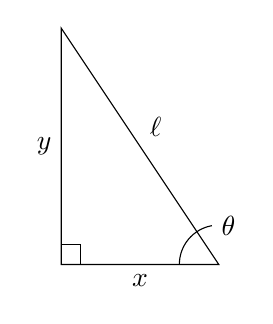
\begin{tikzpicture}
	\draw (0, 0) -- node[anchor=north] {$x$} (2, 0) -- node[anchor=south west] {$\ell$} (0, 3) -- node[anchor=east] {$y$} cycle;
	\draw (0.25, 0) -- (0.25, 0.25) -- (0, 0.25);
	\draw (1.5,0) arc (180:100:0.5) node[anchor=west] {$\theta$};
\end{tikzpicture}
\end{figure}

\begin{align*}
\cos \theta &= x/\ell \\
\theta &= \arccos(x/\ell)
\end{align*}

Now it is easy to find $y$. I could use, for example, the tangent function to relate it to $x$:

\begin{align*}
y/x &= \tan \theta\\
y &= x \tan \theta\\
&= x\tan \arccos(x/\ell)
\end{align*}

This works, the answer is correct. However, you probably know a much quicker, more accurate way to get the answer using Pythagoras:
\begin{align*}
x^2 + y^2 &= \ell^2\\
y &= \sqrt{\ell^2 - x^2}
\end{align*}
In fact we have found a general identity:
\[  x\tan \arccos(x/\ell) = \sqrt{\ell^2 - x^2}. \]
Whenever possible, it would be better to use the square-root method.

In general,  if you have a trig function of an inverse trig function, you can find a better formula which gives the same answer, using Pythagoras. You don't have to memorize all the possible combinations to be able to do this. For example, suppose I have an angle $\theta$ and I know $\tan\theta = a/b$, and I want $\sec\theta$. I could just say $\sec\theta = \sec(\arctan(a/b))$, but that is messy and complicated. Instead, I will just make up a triangle with some convenient side lengths.
\begin{figure}[h!]
\centering
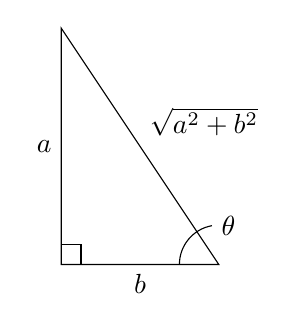
\begin{tikzpicture}
	\draw (0, 0) -- node[anchor=north] {$b$} (2, 0) -- node[anchor=south west] {$\sqrt{a^2+b^2}$} (0, 3) -- node[anchor=east] {$a$} cycle;
	\draw (0.25, 0) -- (0.25, 0.25) -- (0, 0.25);
	\draw (1.5,0) arc (180:100:0.5) node[anchor=west] {$\theta$};
\end{tikzpicture}
\end{figure}

I carefully chose the triangle so that $\tan\theta=a/b$. The triangle doesn't have to correspond to anythign physical, it is just a convenient way to organize my information. Since the secant is always the hypotenuse over the adjacent side, I can just read the answer from the triangle: 
\begin{align*}
\sec(\theta) &= \frac{\sqrt{a^2+b^2}}{b}.
\end{align*}
This gives us a general formula, $\sec(\arctan(a/b)) = \frac{\sqrt{a^2+b^2}}{b}$. 

\end{document}